\documentclass[12pt]{article}
\usepackage[a4paper,left=2.9cm,right=3.0cm,top=1.4cm,bottom=1.2cm]{geometry}
\usepackage{amsmath,amssymb,tikz,eurosym,array,xcolor}
\usetikzlibrary{calc}
\pagestyle{empty}
\setlength{\parindent}{0pt}
\newlength{\tw}\setlength{\tw}{11.4cm}
\newcommand{\loes}[1]{\rlap{\hspace{0.85cm}\small #1}}
\newcommand{\feld}[3][]{\hfill #1\,\rule[-1pt]{2.4cm}{0.4pt}\,\makebox[0.7cm][l]{#2}\loes{#3}}
\newcommand{\nr}[2]{\leavevmode\llap{\makebox[2.05cm][l]{{\footnotesize\color{gray}#1}}}\llap{\textbf{#2.}\hspace{6pt}}}
% Aufgabe mit Feld auf der letzten Textzeile
\newcommand{\AF}[6][]{\par\vspace{10pt plus 1fill}\parbox[b]{\tw}{\raggedright\nr{#1}{#2}#3}\feld[#4]{#5}{#6}}
% Aufgabe ohne Feld (Ankreuzen, Teilaufgaben, Figur folgt)
\newcommand{\AT}[3][]{\par\vspace{10pt plus 1fill}\parbox[t]{\tw}{\raggedright\nr{#1}{#2}#3}\par}
% Teilaufgabe mit Feld
\newcommand{\TF}[5][]{\par\vspace{3pt}\parbox[b]{\tw}{#2}\feld[#1]{#3}{#5}}
\newcommand{\li}[1]{\hfill\rlap{\hspace{\dimexpr\textwidth-\tw+0.85cm\relax}\small #1}}
\newcommand{\lf}{\rule[-1pt]{1.6cm}{0.4pt}}
% Aufgabe links (Text, Teile, Kreuze) mit Figur rechts in der Antwortspalte
\newcommand{\AB}[4][]{\par\vspace{10pt plus 1fill}\parbox[b]{\tw}{\raggedright\nr{#1}{#2}#3}\hfill\parbox[b]{\dimexpr\textwidth-\tw-0.2cm\relax}{\centering #4}}
\newcommand{\op}[2]{{\small #1}\,$\square$\,#2\hspace{1.4em}}
\newcommand{\opz}[1]{\par\vspace{5pt}#1\hfill}
\newcommand{\tipp}[1]{\par\vspace{2pt}{\small\color{gray}Tipp: #1}}
\newcommand{\kopf}[1]{\begin{tikzpicture}[remember picture,overlay]
 \draw[gray,dashed,line width=0.4pt] ($(current page.north east)+(-2.7cm,-1.2cm)$)--($(current page.south east)+(-2.7cm,1.0cm)$);
\end{tikzpicture}%
\llap{\makebox[1.6cm][l]{}}{\bfseries Basis #1}\hfill{\small Erlaubt: Taschenrechner, Formelsammlung, Schmierblatt}\par\vspace{-6pt}}
\newcommand{\rw}{\draw (0.45,0) arc (0:90:0.45); \fill (45:0.22) circle (0.05);}
\begin{document}
%==================================================== Basis 1
\kopf{1}
\AF{1}{Gib 2,5\,h in Minuten an.}{}{min}{150\,min}
\AF{2}{4 Brötchen kosten 1,60\,\euro. Berechne den Preis für 7 Brötchen.}{}{\euro}{2,80\,\euro}
\AF[2026]{3}{Berechne 30\,\% von 70\,\euro.}{}{\euro}{21\,\euro}
\AF[2025]{4}{Ergänze die Hochzahl: \ $850\,000=8{,}5\cdot 10^{\square}$.}{}{}{5}
\AF{5}{Löse die Gleichung $3\cdot(x-4{,}5)=0$.}{$x=$}{}{4,5}
\AT{6}{Kreuze die Figur an, bei der genau $\tfrac14$ der Fläche grau ist.}
\vspace{4pt}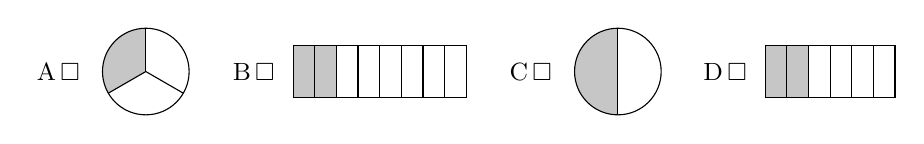
\begin{tikzpicture}[scale=0.55,baseline=(b.base)]
 \node (b) at (0,-0.1) {};
 \node[anchor=east] at (0.1,0) {\small A\,$\square$}; \begin{scope}[shift={(1.4,0)}] \fill[gray!45] (0,0)--(90:1) arc(90:210:1)--cycle; \draw (0,0) circle (1); \foreach \w in {90,210,330} \draw (0,0)--(\w:1); \end{scope}
 \node[anchor=east] at (4.6,0) {\small B\,$\square$}; \begin{scope}[shift={(4.8,-0.6)}] \fill[gray!45] (0,0) rectangle (1,1.2); \foreach \i in {0,...,7} \draw (\i*0.5,0) rectangle +(0.5,1.2); \end{scope}
 \node[anchor=east] at (11.0,0) {\small C\,$\square$}; \begin{scope}[shift={(12.3,0)}] \fill[gray!45] (0,0)--(90:1) arc(90:270:1)--cycle; \draw (0,0) circle (1); \draw (0,-1)--(0,1); \end{scope}
 \node[anchor=east] at (15.5,0) {\small D\,$\square$}; \begin{scope}[shift={(15.7,-0.6)}] \fill[gray!45] (0,0) rectangle (1,1.2); \foreach \i in {0,...,5} \draw (\i*0.5,0) rectangle +(0.5,1.2); \end{scope}
\end{tikzpicture}\hfill\loes{B}
\AT{7}{Mia würfelt fünfmal und erhält die Augenzahlen 2, 6, 1, 6 und 5.}
\TF{a) Ordne die Augenzahlen der Größe nach.}{}{}{1, 2, 5, 6, 6}
\TF{b) Gib den Median an.}{}{}{5}
\AB{8}{Kreuze die Formel für den Umfang $U$ des Rechtecks an.\par\vspace{5pt}\op{A}{$U=x\cdot y$}\op{B}{$U=2x+2y$}\par\vspace{3pt}\op{C}{$U=x+y$}\op{D}{$U=4x$}\li{B}}{\begin{tikzpicture}[scale=0.55]\draw (0,0) rectangle (3.4,1.6);\node[below] at (1.7,0){\small $x$};\node[right] at (3.4,0.8){\small $y$};\end{tikzpicture}}
\AB{9}{Im Dreieck ist der rechte Winkel markiert.\par\vspace{4pt}a) Die Hypotenuse ist die Seite \lf\,.\li{$r$}\par\vspace{4pt}b) Kreuze die Gleichung an, die gilt.\par\vspace{3pt}\op{A}{$r^2=p^2+q^2$}\op{B}{$p^2=q^2+r^2$}\op{C}{$r=p+q$}\li{A}}{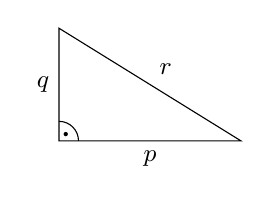
\begin{tikzpicture}[scale=0.55]\draw (0,0)--(4.2,0)--(0,2.6)--cycle;\rw\node[below] at (2.1,0){\small $p$};\node[left] at (0,1.3){\small $q$};\node[above right] at (2.1,1.3){\small $r$};\end{tikzpicture}}
\AT[2026]{10}{Das Viereck ist ein Parallelogramm. Bestimme die Größe des Winkels $\beta$.}
\vspace{2pt}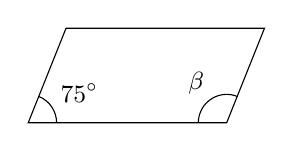
\begin{tikzpicture}[scale=0.6,baseline=(o.base)]
 \coordinate (o) at (0,0); \coordinate (A) at (0,0); \coordinate (B) at (4.2,0); \coordinate (C) at (5.0,2.0); \coordinate (D) at (0.8,2.0);
 \draw (A)--(B)--(C)--(D)--cycle;
 \draw ($(A)+(0.6,0)$) arc (0:68.2:0.6); \node at ($(A)+(30:1.25)$) {\small $75^\circ$};
 \draw ($(B)+(-0.6,0)$) arc (180:68.2:0.6); \node at ($(B)+(128:1.05)$) {\small $\beta$};
\end{tikzpicture}\feld[$\beta=$]{}{$105^\circ$}
\vspace*{\fill}\newpage
%==================================================== Basis 2
\kopf{2}
\AT[2026]{1}{Setze das richtige Zeichen ein: \ $<$, $=$ oder $>$.}
\vspace{2pt}3,5\,m \ \framebox[0.8cm]{\rule{0pt}{0.45cm}} \ 35\,cm\hfill\loes{$>$}
\AF{2}{3 Hefte kosten 2,40\,\euro. Berechne den Preis für 5 Hefte.}{}{\euro}{4,00\,\euro}
\AT{3}{Jeder vierte Schüler kommt mit dem Rad. Kreuze an, wie viel Prozent das sind.}
\vspace{3pt}\op{A}{4\,\%}\op{B}{25\,\%}\op{C}{40\,\%}\op{D}{75\,\%}\hfill\loes{B}
\AF[2026]{4}{Ein Rechteck ist 3,5\,cm lang und 1,5\,cm breit. Berechne den Umfang.}{}{cm}{10\,cm}
\AF{5}{Ein Würfel hat die Kantenlänge 4\,cm. Berechne sein Volumen.}{$V=$}{cm$^3$}{64\,cm$^3$}
\AT{6}{Kreuze an, was für jedes Parallelogramm gilt.}
\vspace{3pt}\op{A}{Alle Winkel sind gleich groß.}\par\vspace{2pt}
\op{B}{Gegenüberliegende Seiten sind parallel.}\hfill\loes{B}\par\vspace{2pt}
\op{C}{Alle Seiten sind gleich lang.}
\AT{7}{Ein Würfel wird einmal geworfen.}
\TF{a) Gib alle Augenzahlen an, die größer als 4 sind.}{}{}{5 und 6}
\TF{b) Gib die Wahrscheinlichkeit für eine Augenzahl größer als 4 an.}{}{}{$\tfrac13$}
\AF[2026]{8}{Berechne den Wert des Terms $5\cdot(x-3)$ für $x=-2$.}{}{}{$-25$}
\AT[2025]{9}{Kreuze an, welcher Wert die Gleichung $x\cdot(x+5)=-6$ erfüllt.}
\vspace{3pt}\op{A}{$2$}\op{B}{$3$}\op{C}{$-2$}\op{D}{$-6$}\hfill\loes{C}
\AB{10}{Das Dreieck hat bei $C$ einen rechten Winkel.\par\vspace{4pt}a) Die Gegenkathete von $\alpha$ ist die Seite \lf\,.\li{$a$}\par\vspace{6pt}b) Gib $\sin\alpha$ als Bruch an: \ $\sin\alpha=$ \lf\li{$\tfrac{a}{c}$}}{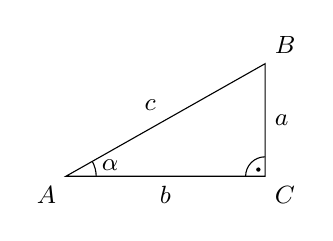
\begin{tikzpicture}[scale=0.55]
 \coordinate (A) at (0,0); \coordinate (C) at (4.6,0); \coordinate (B) at (4.6,2.6);
 \draw (A)--(C)--(B)--cycle;
 \begin{scope}[shift={(C)},rotate=90] \draw (0.45,0) arc (0:90:0.45); \fill (45:0.22) circle (0.05); \end{scope}
 \draw ($(A)+(0.7,0)$) arc (0:29.5:0.7); \node at ($(A)+(14:1.05)$) {\small $\alpha$};
 \node[below left] at (A) {\small $A$}; \node[below right] at (C) {\small $C$}; \node[above right] at (B) {\small $B$};
 \node[below] at (2.3,0) {\small $b$}; \node[right] at (4.6,1.3) {\small $a$}; \node[above left] at (2.3,1.3) {\small $c$};
\end{tikzpicture}}
\vspace*{\fill}\newpage
%==================================================== Basis 3 (schwach)
\large
\setlength{\tw}{11.0cm}
\kopf{3}
\AT[2026]{1}{Kreuze die Figur an, bei der genau $\tfrac13$ der Fläche grau ist.}
\vspace{6pt}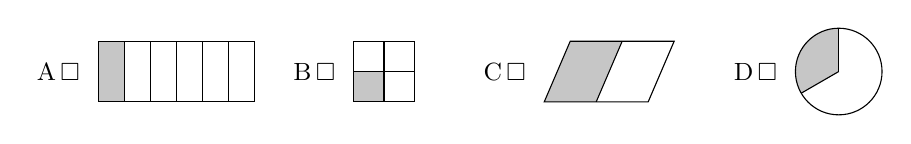
\begin{tikzpicture}[scale=0.55,baseline=(b.base)]
 \node (b) at (0,-0.1) {};
 \node[anchor=east] at (0.1,0) {\small A\,$\square$}; \begin{scope}[shift={(0.3,-0.7)}] \fill[gray!45] (0,0) rectangle (0.6,1.4); \foreach \i in {0,...,5} \draw (\i*0.6,0) rectangle +(0.6,1.4); \end{scope}
 \node[anchor=east] at (6.0,0) {\small B\,$\square$}; \begin{scope}[shift={(6.2,-0.7)}] \fill[gray!45] (0,0) rectangle (0.7,0.7); \draw (0,0) rectangle (1.4,1.4); \draw (0.7,0)--(0.7,1.4); \draw (0,0.7)--(1.4,0.7); \end{scope}
 \node[anchor=east] at (10.4,0) {\small C\,$\square$}; \begin{scope}[shift={(10.6,-0.7)}] \fill[gray!45] (0,0)--(1.2,0)--(1.8,1.4)--(0.6,1.4)--cycle; \draw (0,0)--(2.4,0)--(3.0,1.4)--(0.6,1.4)--cycle; \draw (1.2,0)--(1.8,1.4); \end{scope}
 \node[anchor=east] at (16.2,0) {\small D\,$\square$}; \begin{scope}[shift={(17.4,0)}] \fill[gray!45] (0,0)--(90:1) arc(90:210:1)--cycle; \draw (0,0) circle (1); \draw (0,0)--(90:1); \draw (0,0)--(210:1); \end{scope}
\end{tikzpicture}\hfill\loes{D}
\AT{2}{Jeder zehnte Besucher gewinnt einen Preis. Kreuze an, wie viel Prozent das sind.}
\vspace{4pt}\op{A}{1\,\%}\op{B}{10\,\%}\op{C}{20\,\%}\op{D}{90\,\%}\hfill\loes{B}
\AT{3}{Eine Stunde hat 60 Minuten.}
\TF{a) Gib 2\,h in Minuten an.}{min}{}{120\,min}
\TF{b) Gib 2,5\,h in Minuten an.}{min}{}{150\,min}
\AT{4}{Berechne.}
\TF{a) 10\,\% von 50\,\euro}{\euro}{}{5\,\euro}
\TF{b) 30\,\% von 50\,\euro}{\euro}{}{15\,\euro}
\tipp{10\,\% heißt: durch 10 teilen.}
\AF[2026]{5}{Ein Würfel hat die Kantenlänge 3\,cm. Berechne sein Volumen.}{$V=$}{cm$^3$}{27\,cm$^3$}
\AT{6}{Setze $x=2$ in den Term $4\cdot(x+1)$ ein.}
\TF{a) Schreibe den Term mit der Zahl: \ $4\cdot(\ \square\ +1)$}{}{}{$4\cdot(2+1)$}
\TF{b) Berechne den Wert.}{}{}{12}
\AF{7}{Löse die Gleichung $2\cdot x+3=11$.}{$x=$}{}{4}
\tipp{Rechne zuerst auf beiden Seiten $-3$.}
\vspace*{\fill}
\end{document}
